%! alt Triangle ABC with BC = 300 along the bottom and the altitude from A dropped vertically to H on BC, close to B. The incircle, centred at I, touches BC at D and AB at F, and the altitude crosses it at P and Q with AP = 63, PQ = 112 and QH = 14. The perpendicular from I to the altitude meets it at M, the midpoint of PQ, so M and I are both 70, the inradius, above BC. The tangent AF has length 105.
%! after_paragraph 2
%! scale 1/40
% The shared preamble of every Cevian figure. pipeline/figures turns these colours into theme-aware paint,
% and refuses any other colour, so draw only with them:
%   figink (lines and labels), figaux (construction lines), figaccent (the object the argument turns on),
%   figtint and figaccenttint (light fills).
\documentclass[border=1.5pt]{standalone}
\usepackage{tkz-euclide}
\definecolor{figink}{RGB}{0,0,0}
\definecolor{figaux}{RGB}{85,85,85}
\definecolor{figaccent}{RGB}{192,57,43}
\definecolor{figtint}{RGB}{221,221,221}
\definecolor{figaccenttint}{RGB}{245,213,208}
% tkz-euclide's defaults draw circles, compasses and marks in 50% grey and fill points with a tint.
\makeatletter
\def\tkz@otherlinecolor{figink}
\def\tkz@euc@circlecolor{figink}
\def\tkz@euc@compasscolor{figink}
\def\tkz@euc@mkcolor{figink}
\def\tkz@mk@fill{figink}
\def\tkz@euc@pointfillcolor{figink}
\makeatother
\tkzSetUpLine[color=figink,line width=.7pt]
\tkzSetUpArc[color=figink,line width=.7pt]
\tkzSetUpCompass[color=figink,line width=.5pt]
\tkzSetUpPoint[color=figink,fill=figink,size=3.1pt]
\tikzset{
  every picture/.style={line cap=round,line join=round,color=figink},
  circle style/.append style={color=figink,line width=.7pt},
  aux/.style={color=figaux,line width=.45pt,dash pattern=on 2.6pt off 2pt},
  key/.style={color=figaccent,line width=1pt},
  mk/.style={color=figink,line width=.5pt},
  lbl/.style={color=figink,inner sep=2.2pt},
  len/.style={color=figink,inner sep=1.5pt,font=\small},
}

\begin{document}
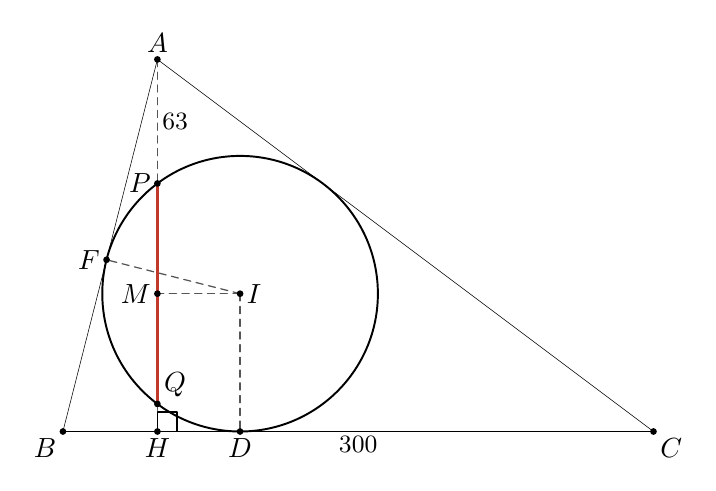
\begin{tikzpicture}
\tkzDefPoint(0.0,0.0){H} %! H = (0, 0)
\tkzDefPoint(0.0,4.7250000){A} %! A = (0, 189)
\tkzDefPoint(-1.2000000,0.0){B} %! B = (-48, 0)
\tkzDefPoint(6.3000000,0.0){C} %! C = (252, 0)
\tkzDefPoint(1.0500000,1.7500000){I} %! I = (42, 70)
\tkzDefPoint(0.0,3.1500000){P} %! P = (0, 126)
\tkzDefPoint(0.0,0.35000000){Q} %! Q = (0, 14)
\tkzDefPoint(0.0,1.7500000){M} %! M = (0, 70)
\tkzDefPoint(1.0500000,0.0){D} %! D = (42, 0)
\tkzDefPoint(-0.64615385,2.1807692){F} %! F = foot(I, A, B)
%! fact perp(A, H, B, C)
%! fact on_circle(P, I, 70)
%! fact on_circle(Q, I, 70)
%! fact tangent(I, 70, B, C)
%! fact tangent(I, 70, A, B)
%! fact tangent(I, 70, A, C)
%! fact midpoint(M, P, Q)
%! fact perp(I, M, A, H)
%! fact dist(A, P) == 63
%! fact dist(P, Q) == 112
%! fact dist(Q, H) == 14
%! fact dist(A, F) == 105
%! fact dist(B, C) == 300
%! fact dist(C, A) == 315
%! fact dist(A, B) == 195
%! fact area(A, B, C) == 28350
%! fact circumradius(A, B, C) == 325/2
\tkzDrawCircle(I,D)
\tkzDrawSegments[aux](A,H I,M I,F I,D)
\tkzDrawPolygon(A,B,C)
\tkzDrawSegment[key](P,Q)
\tkzMarkRightAngle[size=.25,mk](A,H,C)
\tkzDrawPoints(A,B,C,H,I,P,Q,M,D,F)
\tkzLabelPoint[above,lbl](A){$A$}
\tkzLabelPoint[below left,lbl](B){$B$}
\tkzLabelPoint[below right,lbl](C){$C$}
\tkzLabelPoint[below,lbl](H){$H$}
\tkzLabelPoint[right,lbl](I){$I$}
\tkzLabelPoint[left,lbl](P){$P$}
\tkzLabelPoint[above right,lbl](Q){$Q$}
\tkzLabelPoint[left,lbl](M){$M$}
\tkzLabelPoint[below,lbl](D){$D$}
\tkzLabelPoint[left,lbl](F){$F$}
\tkzLabelSegment[right,len](A,P){$63$}
\tkzLabelSegment[below,len](B,C){$300$}
\end{tikzpicture}
\end{document}
